\documentclass[a4paper,12pt]{article}
\usepackage{graphicx}
\usepackage{hyperref}
\usepackage{amsmath}
\usepackage{times}
\usepackage{xcolor}
\usepackage{amsfonts}
\usepackage{garamondx}
\usepackage{framed}  %This is to use the shaded environment
\usepackage{titlesec}


\titlespacing*{\section}
{0pt}{5.5ex plus 1ex minus .2ex}{4.3ex plus .2ex}
\titlespacing*{\subsection}
{0pt}{5.5ex plus 1ex minus .2ex}{4.3ex plus .2ex}

\usepackage{titling}
\setlength{\droptitle}{-8em} 


\textwidth=6.2in
\textheight=8.5in
%\parskip=.3cm
\oddsidemargin=.1in
\evensidemargin=.1in
\headheight=-.3in
\setlength{\parindent}{0pt}



% \renewcommand{\baselinestretch}{1} 
% \setlength{\parskip}{\baselineskip}
% \setlength{\parindent}{0pt}
% \setlength{\marginparwidth}{2.5cm}


\newcommand{\scscst}{\scriptscriptstyle}
\newcommand{\scst}{\scriptstyle}
\newcommand{\Robject}[1]{{\code{#1}}}
\newcommand{\Rfunction}[1]{{\code{#1}}}
\newcommand{\Rclass}[1]{\textit{#1}}
\newcommand{\Rpackage}[1]{\textit{#1}}
\newcommand{\Rexpression}[1]{\code{#1}}
\newcommand{\Rmethod}[1]{{\code{#1}}}
\newcommand{\Rfunarg}[1]{{\code{#1}}}

\newcommand\boldblue[1]{\textcolor{blue}{\textbf{#1}}}
\newcommand\code[1]{\textcolor{red}{\texttt{#1}}}

\usepackage{Sweave}
\begin{document}
\Sconcordance{concordance:1_Stats_Course_Notes-knitr.tex:1_Stats_Course_Notes-knitr.Rnw:%
1 50 1 1 0 5 1 1 7 13 1 1 9 1 1 1 7 160 1 1 5 9 0 1 2 5 1 1 2 1 0 2 1 %
13 0 1 2 8 1 1 2 1 0 1 3 4 0 1 2 3 1 1 4 1 1 1 4 7 0 1 2 8 1}

\definecolor{shadecolor}{gray}{0.95} %this is defining the color of the background in the shaded environment

%\SweaveOpts{concordance=TRUE}



%------------------------------------------------------------
\title{Using R as a Research Tool.\\
Part 2: Basic statistics and report writing.}
%------------------------------------------------------------
\author{Dr Susan Johnston: \href{mailto:Susan.Johnston@ed.ac.uk}{Susan.Johnston@ed.ac.uk}  \\ \\
        Demonstrators: Gergana Daskalova, John Godlee. \\
        Hat-Tips to Kyle Dexter, The Coding Club and R4all.}
%\date{}









\maketitle

%\tableofcontents


%-------------------------------------------
\section {Introduction}
%-------------------------------------------

This practical will follow on from the previous practical in data manipulation and visualisation, exploring how to write reports in \boldblue{R} Markdown and how to conduct simple statistical tests in \boldblue{R}. By the end of the practical, you should be able to:

\begin{itemize}

\item Create data visualisations for statistical tests.
\item Carry out basic statistics, including:

\begin{itemize}

\item Linear regression with \code{lm()}
\item 2-sample t-test with \code{t.test()}
\item Chi-squared test with \code{chisq.test()}

\end{itemize}

\item Write, embed and render code and results into an HTML document.

\end{itemize}




%-------------------------------------------
\section {The basics of R Markdown.}
%-------------------------------------------

\boldblue{R} Markdown is a tool for writing, reproducible reports in \boldblue{R}. It can be used to produce documents with embedded code and figures in HTML, Word and PDF format, and can also be used to create webpages and slideshows.

\subsection{Creating an R Markdown Document.}

Create a new document by going to \textbf{File > New File > R Markdown...}. In the window, name your document, select \textbf{HTML} and click \textbf{OK}. RStudio should automatically create a template as in Figure \ref{fig:MarkdownTemplate}. Don't worry if not - it is saved in the file R\_Markdown\_Template.Rmd. To render the document, click the button that says \textbf{Knit}. You may have to save it first.

\begin{figure}[h]
	\centering 
	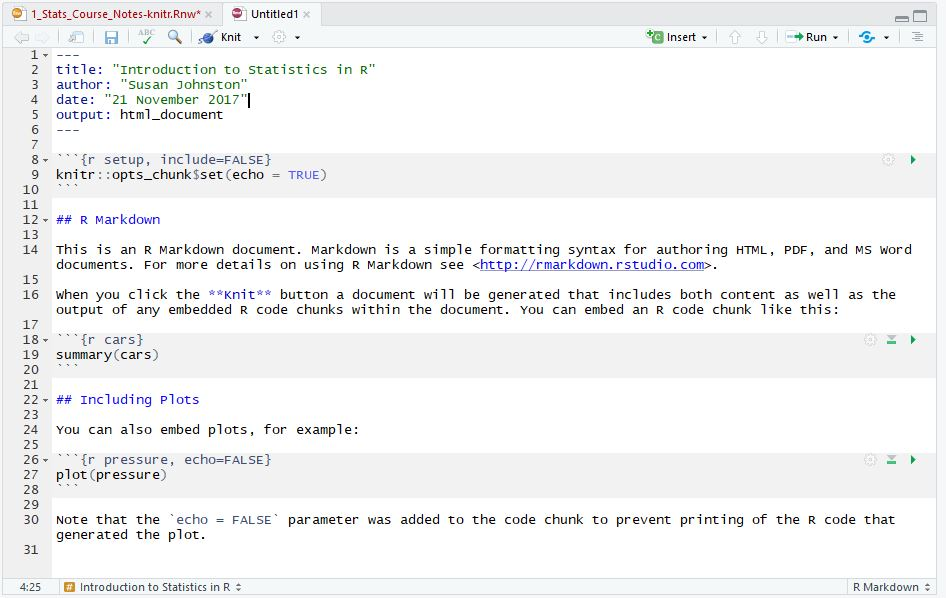
\includegraphics[width=1\textwidth]{figs/MarkdownTemplate.JPG}
	\caption{R Markdown Template.}
	\label{fig:MarkdownTemplate}
\end{figure} 

As you can see



\end{document}

